\documentclass{article}

\usepackage[utf8]{inputenc}
\usepackage{amsthm}
\usepackage{amssymb}
\usepackage{mathtools}
\usepackage{graphicx}
\usepackage{mdframed}
\usepackage{float}
\usepackage[top=0.75in, bottom=0.75in, left=0.75in, right=0.75in]{geometry}
\usepackage{gauss}

\usepackage{array}
\allowdisplaybreaks

\makeatletter
\newcounter{elimination@steps}
\newcolumntype{R}[1]{>{\raggedleft\arraybackslash$}p{#1}<{$}}
\def\elimination@num@rights{}
\def\elimination@num@variables{}
\def\elimination@col@width{}
\newenvironment{elimination}[4][0]
{
    \setcounter{elimination@steps}{0}
    \def\elimination@num@rights{#1}
    \def\elimination@num@variables{#2}
    \def\elimination@col@width{#3}
    \renewcommand{\arraystretch}{#4}
    \start@align\@ne\st@rredtrue\m@ne
}
{
    \endalign
    \ignorespacesafterend
}
\newcommand{\step}[2]
{
    \ifnum\value{elimination@steps}>0\sim\quad\fi
    \left[
        \ifnum\elimination@num@rights>0
            \begin{array}
            {@{}*{\elimination@num@variables}{R{\elimination@col@width}}
            |@{}*{\elimination@num@rights}{R{\elimination@col@width}}}
        \else
            \begin{array}
            {@{}*{\elimination@num@variables}{R{\elimination@col@width}}}
        \fi
            #1
        \end{array}
    \right]
    & 
    \begin{array}{l}
        #2
    \end{array}
    \addtocounter{elimination@steps}{1}
}
\makeatother

\DeclarePairedDelimiter{\abs}{\lvert}{\rvert}
\DeclarePairedDelimiter{\norm}{\lvert \lvert}{\rvert \rvert}

\newtheoremstyle{break}% name
  {}%         Space above, empty = `usual value'
  {}%         Space below
  {\itshape}% Body font
  {}%         Indent amount (empty = no indent, \parindent = para indent)
  {\bfseries}% Thm head font
  {.}%        Punctuation after thm head
  {\newline}% Space after thm head: \newline = linebreak
  {}%         Thm head spec

\newtheorem{Def}{Definition}[section]

\theoremstyle{break}

\newtheorem{innerEx}{Exempel}[section]
\newtheorem{sats}{Sats}[section]
\newtheorem{Rem}{Anmärkning}[]

\newenvironment{Ex}
{\begin{mdframed} \begin{innerEx} \vspace{3pt}}
{\vspace{3pt} \end{innerEx} \end{mdframed}}  

\newenvironment{bevis}
{\begin{mdframed} \begin{proof} \vspace{3pt}}
{\vspace{3pt} \end{proof} \end{mdframed}}

\usepackage{gauss}

\title{
	 Linjär Algebra\\
	 Föreläsning 13 - Determinanter
    \author{Erik Sjöström}
}
\begin{document}
\maketitle
\section{Terminologi} % (fold)
\label{sec:terminologi}
\begin{itemize}
	\item $n! = n \cdot (n-1) \cdot ... \cdot 1$
	\begin{Ex}
	    \begin{gather*}
	    	3! = 3 \cdot 2 \cdot 1\\
	    	25! = 25 \cdot 24 \cdot ... \cdot 2 \cdot 1 \approx 1.5 \cdot 10^{25}
	    \end{gather*}
	\end{Ex}
	\item Permutation är en uppräkning av \{1,2,3,...,n\} i en given ordning.
	\begin{Ex}
	    Det $3!$ möjliga permutationerna av \{1,2,3\} nämligen:
	    \begin{align*}
	    &&\{1,2,3\}
	    &&\{1,3,2\}
	    &&\{2,1,3\}
	    &&\{2,3,1\}
	    &&\{3,1,2\}
	    &&\{3,2,1\}
	    \end{align*}
	\end{Ex}
	\item En permutation kallas udda om det krävs ett udda antal platsbyten för att överföra den till \{1,2,...,n\}, annars jämn.
	\begin{Ex}
	    \begin{align*}
	    &&\mbox{Jämn}
	    &&\mbox{Udda}
	    &&\mbox{Udda}
	    &&\mbox{Jämn}
	    &&\mbox{Jämn}
	    &&\mbox{Udda}
	    \\
	    &&\{1,2,3\}
	    &&\{1,3,2\}
	    &&\{2,1,3\}
	    &&\{2,3,1\}
	    &&\{3,1,2\}
	    &&\{3,2,1\}
	    \end{align*}
	\end{Ex}
\end{itemize}
% section terminologi (end)
Låt $A_{n \times n}$ vara en $2 \times 2$-matris:
\[
    \mathbf{A} = \begin{bmatrix} a_{11}&a_{12}\\a_{21}&a_{22} \end{bmatrix}
\]
\[
\begin{array}{c|c|c}
	\mbox{Möjliga produkter:} & \mbox{Permutation av kolumnindex:} & \mbox{Udda/jämn permutation:}\\\hline
	a_{11} \cdot a_{22} & \{1,2\} & \mbox{Jämn} \\\hline
	a_{12} \cdot a_{21} & \{2,1\} & \mbox{Udda}\\\hline
\end{array}
\]
\[
    \mathbf{det}(\mathbf{A}) = a_{11} \cdot a_{22} - a_{21} \cdot a_{12}
\]
\begin{Ex}
    \begin{center}
    	Här fattas det ett exempel eftersom Blom ej har lagt upp det på hemsidan än.	
    \end{center}
\end{Ex}
Vi ser från determinanten av en matris \textbf{A} att:
\begin{itemize}
	\item Om \textbf{A} innehåller en rad eller kolumn med bara nollor blir \textbf{det}(\textbf{A}) = 0
	\item \textbf{det}(\textbf{A}) = \textbf{det}(\textbf{A}$^T$)
	\item Om \textbf{A} är triangulär:
	\begin{align*}
	&&	\mathbf{A} = 
	    \begin{bmatrix}
	    d_1 & ... & x\\
	    \vdots & \ddots & \vdots\\
	    0 & ... & d_n
	    \end{bmatrix}
	&&\mbox{eller}
	&& 	\mathbf{A} = 
	    \begin{bmatrix}
	    d_1 & ... & 0\\
	    \vdots & \ddots & \vdots\\
	    x & ... & d_n
	    \end{bmatrix}
	\end{align*}
	så är \textbf{det}(\textbf{A}) = produkten av diagonalelementent.
\end{itemize}
För att beräkna \textbf{det}(\textbf{A}$_{n \times n}$) behöver vi utfära cirka $n!$ multiplikationer och additioner.
\begin{Ex}
    $A_{25 \times 25}$. Det behövs cirka $25! \approx 1.5 \cdot 10^{25}$ operationer. Antag att en dator utför $10^{12}$ operationer/sekund då tar det cirka 500 tusen år att beräkna.
\end{Ex}
Lösningen på detta problem är att radreducera (Gausseliminera) innan man beräknar \textbf{det}(\textbf{A}).\\
Låt \textbf{A} och \textbf{B} vara två $(n \times n)$-matriser och \textbf{B} vara resultatet av precis \underline{en} radoperation på \textbf{A}. Resultat beroende på operation blir:
\begin{itemize}
	\item Addition: $\mathbf{det}(\mathbf{B}) = \mathbf{det}(\mathbf{A})$
	\item Platsbyte: $\mathbf{det}(\mathbf{B}) = -\mathbf{det}(\mathbf{A})$
	\item Skalning med \textit{k}: $\mathbf{det}(\mathbf{B}) = k \cdot \mathbf{det}(\mathbf{A})$
\end{itemize}
\begin{Ex}
	Beräkna:
	\[
	\begin{gmatrix}[v]
		1 & 2 & 3\\
		-2 & 0 & 1\\
		0 & 4 & 2
		\rowops
			\add[2]{0}{1}
	\end{gmatrix} = 
	\begin{gmatrix}[v]
		1 & 2 & 3\\
		0 & 4 & 7\\
		0 & 4 & 2
		\rowops
			\add[-1]{1}{2}
	\end{gmatrix} =
	\begin{gmatrix}[v]
		1 & 2 & 3\\
		0 & 4 & 7\\
		0 & 0 & -5
	\end{gmatrix} =
	1 \cdot 4 \cdot (-5) = - 20
	\]
\end{Ex}
Antalet operationer (mul, add, subtr) som behövs för Gausseliminering av en $(n \times n)$-matris är cirka $2n^3/3$.
\begin{Ex}
	Radreduceringen av en $(25 \times 25)$-matris blir $2 \cdot 25^3/3 \approx 10.000$ operationer, vilket tar mindre än 1 sekund.
\end{Ex}
Låt $\mathbf{A}_{n \times n}$ gausselimineras till övertriangulär form:
\[
\begin{bmatrix}
	d_1 & ... & x\\
	\vdots & \ddots & \vdots\\
	0 & ... & d_n
\end{bmatrix}
\]
med hjälp av addition och platsbyte. Då har vi att:
\[
\mathbf{det}(\mathbf{A}) = (-1)^r \cdot d_1 \cdot d_2 \cdot ... \cdot d_n
\]
där \textit{r} är antalet platsyten.\\
Om \textbf{A} ej är inverterbar så kommer minst ett av diagonalelementen att vara 0 (ty \textbf{A} ej har pivotelement i varje kolumn) $\Rightarrow \mathbf{det}(\mathbf{A}) = 0$\\
Om \textbf{det}(\textbf{A}) = 0, så måste något av diagonalelementen vara 0, dvs \textbf{A} har ej pivotelement i varje kolumn, dvs \textbf{A} är ej inverterbar.

\begin{center}
	\underline{\textbf{A} inverterbar $\Leftrightarrow$ $\mathbf{det}(\mathbf{A}) \neq 0$}
\end{center}
\newpage
\begin{sats}
	Det gäller också att, om \textbf{A} och \textbf{B} är $(n \times n)$-matriser:
	\[
	\mathbf{det}(\mathbf{A} \cdot \mathbf{B}) = \mathbf{det}(\mathbf{A}) \cdot \mathbf{det}(\mathbf{B})
	\]
\end{sats}
\section{Area, volymskala} % (fold)
\label{sec:area_volymskala}
Kom ihåg (F6). Låt $\mathbf{A}_{2 \times 2} = \begin{bmatrix} \vec{a}_1 & \vec{a}_2 \end{bmatrix}$\\
Arean av parallellogrammet som spänns upp av $\vec{a}_1$, $\vec{a}_2$ är: $\abs{\mathbf{det}(\mathbf{A})}$
\begin{center}
	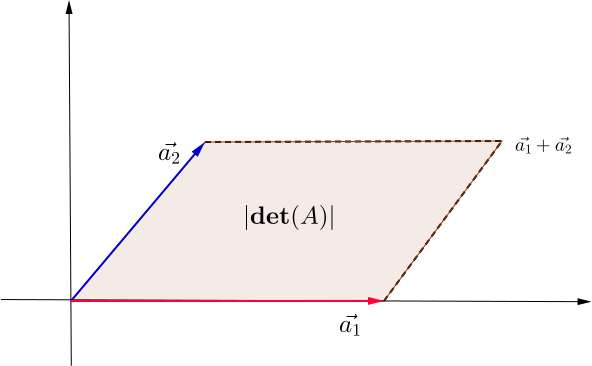
\includegraphics[scale=0.5]{areagram.png}
\end{center}
\begin{Ex}
	Bestäm arean av området vars hörn är:
	\begin{align*}
	&(-2,-2)
	&&(0,3)
	&&(4,-1)
	&&(6,4)
	\end{align*}
	\begin{center}
		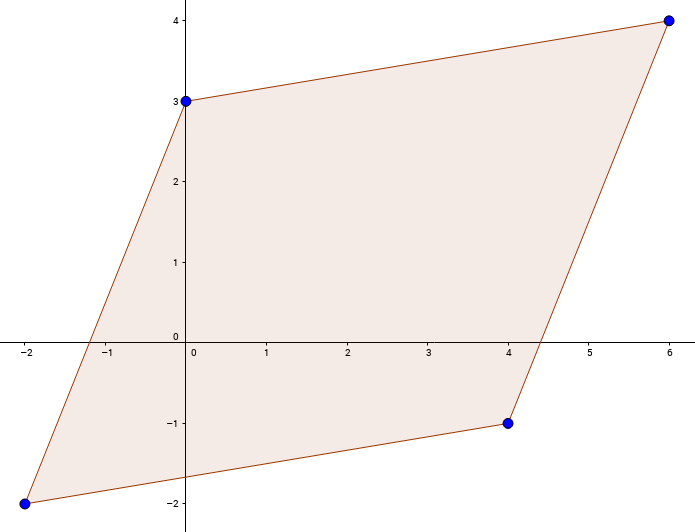
\includegraphics[scale=0.3]{gram.png}
	\end{center}
	För att kunna beräkna arean mha determinanter måste vi translatera (flytta) parallellogrammet så att ett av hörnen hamnar i origo (0,0).
	\newpage
	Vi translaterar med $\vec{t} = \begin{bmatrix} 2\\2 \end{bmatrix}$. Vi får:
	\begin{align*}
	&(0,0)
	&&(2,5)
	&&(6,1)
	&&(8,6)
	\end{align*}
	\begin{center}
		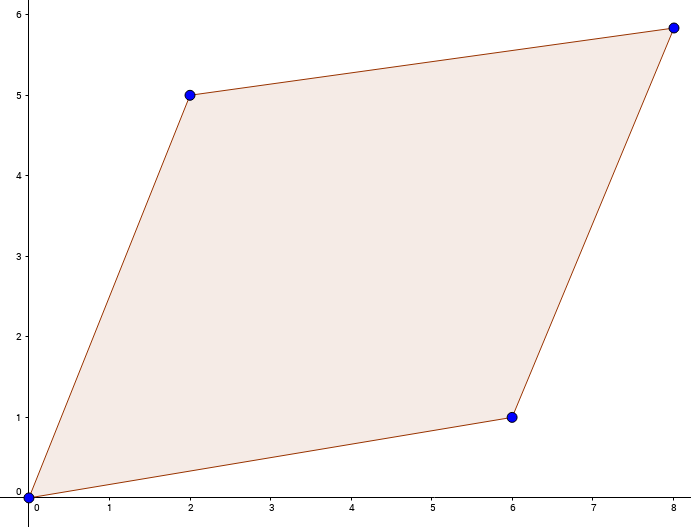
\includegraphics[scale=0.3]{origogram.png}
	\end{center}
	\underline{Arean är oförändrad}
	\[
	\mathbf{A} = \begin{bmatrix} \vec{a}_1&\vec{a}_2 \end{bmatrix} = \begin{bmatrix} 2&6\\5&1 \end{bmatrix}
	\]
	Parallellogrammet som spänns upp av $\vec{a}_1$ och $\vec{a}_2$ består av alla punkter:
	\[
	\{s \cdot \vec{a}_1 + t \cdot \vec{a}_2: 0 \le s \le 1, 0 \le t \le 1\}
	\]
\end{Ex}
\newpage
\noindent
Låt $f: \mathbb{R}^2 \rightarrow \mathbb{R}^2$ vara en linjär transformation $f(\vec{x}) = \mathbf{A} \cdot \vec{x}$.\\
Låt $\mathbf{D}: \{s \cdot \vec{d}_1 + t \cdot \vec{d}_2: 0 \le s \le 1, 0 \le t \le 1\}$ vara ett paralellogram i $\mathbb{R}^2$.\\
Vad blir arean av $f(\mathbf{D})$? (arean av $\mathbf{D} = \abs{\mathbf{det}(\begin{bmatrix} \vec{d}_1 & \vec{d}_2 \end{bmatrix})}$)
\[
f(\mathbf{D}) = f(s \cdot \vec{d}_1 + t \cdot \vec{d}_2) = s \cdot f(\vec{d}_1) + t \cdot f(\vec{d}_2) = \overbrace{s \cdot \mathbf{A} \cdot \vec{d}_1 + t \cdot \mathbf{A} \cdot \vec{d}_2}^\text{Parallellogram}
\]
\begin{gather*}
	\mbox{Arean av }f(\mathbf{D}) = \abs{\mathbf{det}(\begin{bmatrix} \mathbf{A} \cdot \vec{d}_1 & \mathbf{A} \cdot \vec{d}_2 \end{bmatrix})} = \\
	\mbox{\textbf{Obs: }} \begin{bmatrix} \mathbf{A} \cdot \vec{d}_1 & \mathbf{A} \cdot \vec{d}_2 \end{bmatrix} = \mathbf{A} \cdot \begin{bmatrix} \vec{d}_1 & \vec{d}_2 \end{bmatrix}\\
	= \abs{\mathbf{det}(\mathbf{A} \cdot 
	\begin{bmatrix}
	\vec{d}_1 & \vec{d}_2
	\end{bmatrix})} = \abs{\mathbf{det}(\mathbf{A}) \cdot \mathbf{det}(\begin{bmatrix} \vec{d}_1 & \vec{d}_2 \end{bmatrix})} = \abs{\mathbf{det}(\mathbf{A})} \cdot \mbox{"arean av \textbf{D}"}
\end{gather*}
\begin{Ex}
	Låt \textbf{D} vara parallellogrammet som spänns upp av:
	\begin{align*}
	&\begin{bmatrix} 1\\3 \end{bmatrix}
	&&\begin{bmatrix} 5\\1 \end{bmatrix}
	\end{align*}
	Låt $f: \mathbb{R}^2 \rightarrow \mathbb{R}^2$ och:
	\[
	f(\vec{x}) = \begin{bmatrix} 1&-1\\0&2 \end{bmatrix}\begin{bmatrix} x_1\\x_2 \end{bmatrix}
	\]
	Bestäm arean av bilden av \textbf{D} (\textit{f}(\textbf{D})):\\
	\textbf{Lösning:}
	\begin{gather*}
		\mbox{"Arean av \textit{f}(\textbf{D})"} = \abs{\mathbf{det}(\mathbf{A})} \cdot \mbox{"Arean av \textbf{D"}}\\
		\mathbf{det}(\mathbf{A}) = \abs{1 \cdot 2 - 0 \cdot (-1)} = 2\\
		\mbox{"Arean av \textbf{D}"} = \abs{\mathbf{det}(\begin{bmatrix} 1&5\\3&1 \end{bmatrix})} = \abs{1 \cdot 1 - 3 \cdot 5} = \abs{-14} = 14\\
		\mbox{"Arean av \textit{f}(\textbf{D})"} = 2 \cdot 14 = 28
	\end{gather*}
\end{Ex}
\begin{Ex}
	Låt $\mathbf{f}: \mathbb{R}^2 \rightarrow \mathbb{R}^2$ vara rotationen motsols med $\theta$, dvs:
	\[
	f(\vec{x}) = \overbrace{\begin{bmatrix} \cos(\theta) & -\sin(\theta)\\\sin(\theta)&\cos(\theta) \end{bmatrix}}^{\mathbf{A}} \cdot \begin{bmatrix} x_1\\x_2 \end{bmatrix}
	\]
	\[
	\mathbf{det}(\mathbf{A}) = \cos^2(\theta) -(-\sin^2(\theta)) = \cos^2(\theta) + \sin^2(\theta) = 1
	\]
	Dvs: rotation förändrar inte arean.
\end{Ex}
% section area_volymskala (end)
\end{document}










